\documentclass{article}
%Package linking and settings.
\usepackage[utf8]{inputenc}
\usepackage[russian]{babel}
\usepackage{amsmath,amssymb}
\usepackage{graphics}
\usepackage{gensymb}
\usepackage{pbox}
\usepackage{physics}
\usepackage{mathrsfs}
\usepackage{float}
\usepackage{tikz, tkz-fct, pgfplots}
\usepgfplotslibrary{polar}
\pgfplotsset{compat=1.15}
\usetikzlibrary{arrows}
\usepackage{geometry}
\geometry{
	a4paper,
	total={170mm,257mm},
	left=20mm,
	top=20mm
} 
\usepackage{hyperref}
\usepackage{longtable}
\usepackage{textcomp}
\usepackage{booktabs}
\newcolumntype{x}[1]{>{\centering\arraybackslash\hspace{0pt}}m{#1}}
% \newcolumntype{C}{ >{\centering\arraybackslash} m{4cm} }
\renewcommand{\arraystretch}{1.4}
\usepackage{cellspace}
\setlength\cellspacetoplimit{4pt}
\setlength\cellspacebottomlimit{4pt}

\newcommand\cincludegraphics[2][]{\raisebox{-0.5\height}{\includegraphics[#1]{#2}}}

\usepackage[labelsep=period]{caption}
% \usepackage{subfig}
\usepackage{subcaption}

\makeatletter 
% \newcommand\semiLarge{\@setfontsize\semiLarge{13.14}{15.77}}
\newcommand\semiLarge{\@setfontsize\semiLarge{13.20}{15.84}}
\makeatother

\usepackage{titlesec}
\titleformat{\section}
 [hang]
 {\normalfont\bfseries\LARGE}
 {\arabic{section}}
 {0.8em}
 {}
\renewcommand{\thesection}{\arabic{section}}
\titleformat{\subsection}
 [hang]
 {\normalfont\bfseries\semiLarge}
 {\arabic{section}.\arabic{subsection}}
 {0.8em}
 {}
\renewcommand{\thesubsection}{\arabic{section}.\arabic{subsection}}
\renewcommand{\thesubsubsection}{\arabic{section}.\arabic{subsection}.\arabic{subsubsection}}
\newcommand\tline[2]{$\underset{\text{#1}}{\text{\underline{\hspace{#2}}}}$}

\pagenumbering{arabic}

\def\doubleunderline#1{\underline{\underline{#1}}}
\DeclareMathOperator{\di}{d\!}

% \usepackage{mathtools}
%     \newtagform{lbl}[\renewcommand{\theequation}{(\arabic{subsection}.\arabic{equation})}]{}{}
%     \usetagform{lbl}
%     \counterwithin*{equation}{subsection}
%     \renewcommand{\theequation}{(\arabic{subsection}.\arabic{equation})}

\usepackage{mathtools}
    \newtagform{lbl}[\renewcommand{\theequation}{(\arabic{equation})}]{}{}
    \usetagform{lbl}
    \renewcommand{\theequation}{(\arabic{equation})}

\usepackage{fontsize}
  \changefontsize[12.8pt]{11pt}

\makeatletter
\renewenvironment{bmatrix}
  {\left[\mkern3.5mu\env@matrix}
  {\endmatrix\mkern3.5mu\right]}

\renewenvironment{vmatrix}
  {\left\lvert\mkern5mu\env@matrix}
  {\endmatrix\mkern5mu\right\rvert}
\makeatother

\makeatletter
\newenvironment{sqcases}{%
  \matrix@check\sqcases\env@sqcases
}{%
  \endarray\right.%
}
\def\env@sqcases{%
  \let\@ifnextchar\new@ifnextchar
  \left\lbrack
  \def\arraystretch{1.2}%
  \array{@{}l@{\quad}l@{}}%
}
\makeatother

\captionsetup{width=0.8\textwidth, justification=centerlast}
% \renewcommand{\thesubfigure}{\Roman{subfigure}}

\usepackage{listings}
\usepackage{xcolor}
\definecolor{codegreen}{rgb}{0,0.6,0}
\definecolor{codegray}{rgb}{0.5,0.5,0.5}
\lstdefinestyle{mystyle}{
    numberstyle=\color{codegray},
    commentstyle=\color{codegreen},
    numbers=left,                    
    numbersep=15pt,
    breakatwhitespace=true,
    breaklines=true, 
    basicstyle=\ttfamily\normalsize
}
\lstset{style=mystyle}


\begin{document}





\pagestyle{empty}
\centerline{\large Министерство науки и высшего образования}	
\centerline{\large Федеральное государственное бюджетное образовательное}
\centerline{\large учреждение высшего образования}
\centerline{\large ``Московский государственный технический университет}
\centerline{\large имени Н.Э. Баумана}
\centerline{\large (национальный исследовательский университет)''}
\centerline{\large (МГТУ им. Н.Э. Баумана)} \vspace{0.3cm}
\hrule
\vspace{2cm}
\begin{figure}[h]
\center
\includegraphics[height=0.4\linewidth]{gerb.png}
\end{figure}
\begin{center}
	\large	
	\begin{tabular}{c}
		Факультет ``Фундаментальные науки'' \\
		Кафедра ``Высшая математика''		
	\end{tabular}
\end{center}
\vspace{1.4cm}
\begin{center}
	\begin{tabular}{c}
		{\LARGE \bf Курсовая Работа} \vspace{0.4cm} \\
		{\Large \bf Построение фазового портрета динамической} \\
		{\Large \bf системы на плоскости} \vspace{0.4cm}
	\end{tabular}
\end{center}
\vspace{0.3cm}
\begin{center} \large
\begin{tabular}{ m{6.6cm} m{3.8cm} m{3.6cm}}
 Студент группы ФН1-41Б & \tline{\it(Подпись, дата)}{3.3cm} & Гвоздев П.А. \\[0.6cm]
 Руководитель курсового проекта & \tline{\it(Подпись, дата)}{3.3cm} & Филиновский А.В.
\end{tabular}
\end{center}
\vspace{0.18cm}
\vfill
\begin{center}
	\large	
	\begin{tabular}{c}
		Москва\\
		2024
	\end{tabular}
\end{center}









\setlength{\jot}{5pt}
\centerline{\large Министерство науки и высшего образования}	
\centerline{\large Федеральное государственное бюджетное образовательное}
\centerline{\large учреждение высшего образования}
\centerline{\large ``Московский государственный технический университет}
\centerline{\large имени Н.Э. Баумана}
\centerline{\large (национальный исследовательский университет)''}
\centerline{\large (МГТУ им. Н.Э. Баумана)}
\vspace{0.3cm}
\hrule
\vspace{1.4cm}
\begin{flushright}
\begin{tabular}{m{8cm}}
    \centering УТВЕРЖДАЮ \\[10pt]
    Заведующий кафедрой \hfill \tline{\it(Индекс)}{3.7cm} \\[8.5pt]
    \tline{\it(Ф.И.О.)}{8cm} \\[7.5pt]
    \guillemotleft \tline{}{2.0cm} \hspace{-5pt}\guillemotright \hfill \tline{}{4.0cm}\;\; 2024 г.
\end{tabular}
\end{flushright}
\vspace{1.6cm}

\begin{center}
    \huge \bf Задание
\end{center}
\vspace{0.4cm}

\begin{flushleft} \large
По дисциплине дифференциальные уравнения\\
Cтудент группы ФН1–41Б, Гвоздев Платон Алексеевич\\
Вариант задания: 1\\
Тема: \guillemotleft Построение фазового портрета динамической системы на плоскости \hspace{-3pt}\guillemotright\\
Направленность: учебная\\
Источник тематики: кафедра \guillemotleft Высшая математика \hspace{-3pt}\guillemotright\; (ФН1)\\
График выполнения: 25\% к \underline{\hspace{{10pt}}} неделе, 50\% к \underline{\hspace{{10pt}}} неделе, 75\% к \underline{\hspace{{10pt}}} неделе, 100\% к \underline{\hspace{{10pt}}} неделе\\
Техническое задание: Исследовать динамическую систему и построить ее фазовый портрет\\
Оформление: расчетно–пояснительная работа на 20–ти листах А4\\
Перечень графического материала (чертежи, плакаты, слайды и т. п.):
графики фазовых портретов, программный код\\
\vspace{1.5cm}
Дата выдачи задания \guillemotleft 11 \hspace{-3pt}\guillemotright\  марта 2024 г.
\vspace{1.2cm}

\begin{tabular}{ m{6.6cm} m{3.8cm} m{3.6cm}}
Студент группы ФН1-41Б & \tline{\it(Подпись, дата)}{3.3cm} & Гвоздев П.А. \\[0.6cm]
Руководитель курсового проекта & \tline{\it(Подпись, дата)}{3.3cm} & Филиновский А.В.
\end{tabular}

\end{flushleft}

\newpage



\pagestyle{plain}
\setcounter{page}{3}
{ \large
\tableofcontents
}
\newpage
\section{Введение}
Дифференциальные уравнения (ДУ) — раздел математики, в котором изучаются теория и
способы решения уравнений и систем уравнений, содержащих искомую функцию и ее производные разных порядков от одного аргумента (обыкновенные ДУ) или от нескольких аргументов (ДУ в частных производных). В самих уравнениях может находиться не только неизвестная функция, но и различные её производные. Такими уравнениями описывается связь между неизвестной функцией и ее производными. Подобные связи отыскиваются в различных областях знаний: в механике, физике, химии, биологии, экономике и т. д. На практике дифференциальные уравнения применяются для описания природных явлений математическим способом.
Так, например, в  физике многие законы можно описать с помощью различных ДУ.\par
Важным разделом теории ДУ является теория устойчивости - дисциплина, изучающая закономерности поведения систем под действием внешних воздействий. Математическая теория устойчивости изучает поведение решений системы ДУ при $t\xrightarrow{}\infty$. Одно из основных направлений исследований - определение случаев, когда можно утверждать, что решения системы ДУ мало меняются на всём бесконечном интервале $t_0\leq t < \infty$ при любых достаточно малых изменениях начальных условий и функций, входящих в уравнения рассматриваемой системы.\par
В прикладном своём аспекте теория устойчивости нашла наибольшее применение при изучении устойчивости механических систем. Так, множество задач таких как расчёт траекторий движения, управления движением, оценка стабильности динамического процесса, предполагают рассмотрение и исследование на устойчивость решений некоторой системы ДУ, описывающей конкретный процесс. Во многих случаях осуществляется поиск положений устойчивого и неустойчивого равновесия системы.
Достаточное представление об устойчивости решений системы в координатной области (где координаты – переменные, зависящие от $t$) даёт фазовый портрет или множество интегральных
кривых системы в этой области.\par
В данной работе рассмотрены 2 системы дифференциальных уравнений 1–го порядка
и построены фазовые портреты соответствующих систем в области, содержащей их особые
точки. Графическая и кодовая реализация решений ДУ будет представлена при помощи соответствующих библиотек языка программирования Python.

\newpage



\section{Теоретическая часть}
Рассмотрим нормальную систему из $n$ дифференциальных уравнений
\begin{equation}
    \dfrac{d\Vec{x}}{dt} = \Vec{F}(t,\Vec{x}),  \text{ где} \quad \vec{x}(t)=(x_1,...,x_n)^T, \quad \vec{F}=(F_1,...,F_n)^T. \label{eq:theory1}
\end{equation}
Решение $x = g(t)$ с начальным условием $x(t_0) = x_0$ называется устойчивым по Ляпунову, если 
\begin{equation*}
\forall\, \varepsilon >0\;\; \exists\,\delta = \delta(\varepsilon)>0\, :\,
\lVert \tilde{x}_0 - x_0\rVert < \delta \implies \lVert \tilde{x}(t) - g(t) \rVert < \varepsilon,\; \forall t>t_0, 
\end{equation*}
где $\tilde{x}(t)$ решение с начальным условием $\tilde{x}(t_0)=\tilde{x}_0$. Таким образом, каждое решение с начальным условием из $\delta$-окрестности точки $x_0$ при $t_0 \leq t < \infty$ существует и не выходит из $\varepsilon$-трубки, ось которой -- решение $x = g(t)$.\par
Решение $x = \varphi(t)$ называется асимптотически устойчивым по Ляпунову, если оно устойчиво по Ляпунову и выполняется следующее условие:
\begin{equation*}
    \exists\, \sigma >0\,:\, \lVert \tilde{x}_0 - x_0\rVert < \sigma \implies \lim_{t\rightarrow\infty} \lVert \tilde{x}(t) - \varphi(t) \rVert =0.
\end{equation*}
Обыкновенные дифференциальные уравнения, входящие в систему вида \ref{eq:theory1}, называют уравнениями возмущенного движения. Решение системы \ref{eq:theory1}, исследуемое на устойчивость, называют невозмущенным движением.\par
Особая точка –- решение системы дифференциальных уравнений или точка, в которой функция постоянна. Пусть дана автономная система дифференциальных уравнений $\dot{x} = F(x)$ с начальными условиями $F(0) = 0$, где вектор-функция $F(x)$ дважды непрерывно дифференцируема в окрестности начала координат. Эта функция в силу непрерывной дифференцируемости представима в виде
\begin{equation} \label{eq:theory2}
    F(x) = Ax + \Phi(x),\;\;\text{где} \quad \lVert \Phi(x) \rVert = o\left(\lVert x\rVert\right), \;\; x\rightarrow0.
\end{equation}
Преобразовывая и отбрасывая бесконечно малые слагаемые в формуле \ref{eq:theory2}, мы получаем выражение для первого приближения системы $\dot{x} = F(x)$ в окрестности начала координат:
\begin{equation} \label{eq:theory3}
    \dfrac{dx}{dt} = Ax, \;\;\text{где} \;\; A=\textrm{const}.
\end{equation}
\vspace{-0.3cm}
\subsection{Первая теорема Ляпунова}
Если все корни характеристического уравнения матрицы $A$ системы уравнений первого приближения \ref{eq:theory3} имеют отрицательную действительную часть, то невозмущённое движение $x(t)\equiv0$ асимптотически устойчиво независимо от вида слагаемого $\Phi(x)$:
\begin{equation*}
    \textrm{Re}(\lambda_j) < 0,\;\; \forall \lambda_j \,:\, \textrm{det}(A-\lambda_jE) = 0
    \quad \implies\quad  x(t)\equiv 0 \;\text{ -- \;асимптотически устойчиво.}
\end{equation*}
\subsection{Вторая теорема Ляпунова}
Если среди корней характеристического уравнения матрицы $A$ системы уравнений первого приближения \ref{eq:theory3} имеется хотя бы один корень с положительной действительной частью, то невозмущённое движение $x(t)\equiv0$ неустойчиво независимо от вида слагаемого $\Phi(x)$:
\begin{equation*}
    \exists\, \lambda_k\,:\, (\,\textrm{Re}(\lambda_k) > 0\,)\land (\,\textrm{det}(A-\lambda_kE) = 0\,)
    \quad \implies\quad  x(t)\equiv 0 \;\text{ -- \;неустойчиво.}
\end{equation*}
\subsection{Критерий асимптотической устойчивости линейной однородной системы}
Для асимптотической устойчивости нормальной линейной однородной системы обыкновенных дифференциальных уравнений с постоянными коэффициентами \ref{eq:theory3} необходимо и достаточно, чтобы все корни характеристического уравнения матрицы $A$ системы имели отрицательную действительную часть.
\newpage
\subsection{Фазовые траектории положения равновесия линейной однородной\\ системы ДУ с постоянными коэффициентами}

\begin{longtable}[c]{|c|x{3.0cm}|x{3.0cm}|Sc|x{3.0cm}|}
\hline
\textnumero & Корни характер. уравнения & Точка покоя & Фазовый портрет & Уст.\,/\,неуст. тривиального решения\\ \hline
\endhead
1 & $\lambda_1 \neq \lambda_2$ \par $\lambda_1 > 0$ \par $\lambda_2 > 0$ & Неустойчивый узел &
\cincludegraphics[width=5.2cm]{Images/Graphs/Table/Graph1.png} & Неустойчиво \\ \hline
2 & $\lambda_1 \neq \lambda_2$ \par $\lambda_1 < 0$ \par $\lambda_2 < 0$ & Устойчивый узел &
\cincludegraphics[width=5.2cm]{Images/Graphs/Table/Graph2.png} & Асимптотически устойчиво \\ \hline
3 & $\lambda_1 \neq \lambda_2$ \par $\lambda_1 > 0$ \par $\lambda_2 < 0$ & Седло &
\cincludegraphics[width=5.2cm]{Images/Graphs/Table/Graph3.png} & Неустойчиво \\ \hline
4 & $\lambda_{1,2} = \pm i\beta$ & Центр &
\cincludegraphics[width=5.2cm]{Images/Graphs/Table/Graph4.png} & Устойчиво по Ляпунову \\ \hline
5 & $\lambda_{1,2} = \alpha\pm i\beta$ \par $\alpha > 0$ & Неустойчивый фокус &
\cincludegraphics[width=5.2cm]{Images/Graphs/Table/Graph5.png} & Неустойчиво \\ \hline
6 & $\lambda_{1,2} = \alpha\pm i\beta$ \par $\alpha < 0$ & Устойчивый фокус &
\cincludegraphics[width=5.2cm]{Images/Graphs/Table/Graph6.png} & Асимптотически устойчиво \\ \hline
7.1 & $\lambda_1 = \lambda_2$ \par $\lambda_1 > 0$ \par Искл. 7.2 & Неустойчивый вырожденный узел &
\cincludegraphics[width=5.2cm]{Images/Graphs/Table/Graph7_1.png} & Неустойчиво \\ \hline
7.2 & $\begin{cases} \;\dot{x} = ax, \\ \;\dot{y} = ay; \end{cases}$ \par\;\par \hspace{-4pt}$a\,>\,0$ & Неустойчивый дикритический узел &
\cincludegraphics[width=5.2cm]{Images/Graphs/Table/Graph7_2.png} & Неустойчиво \\ \hline
8.1 & $\lambda_1 = \lambda_2$ \par $\lambda_1 < 0$ \par Искл. 8.2 & Устойчивый вырожденный узел &
\cincludegraphics[width=5.2cm]{Images/Graphs/Table/Graph8_1.png} & Асимптотически устойчиво \\ \hline
8.2 & $\begin{cases} \;\dot{x} = ax, \\ \;\dot{y} = ay; \end{cases}$ \par\;\par \hspace{-4pt}$a\,<\,0$ & Устойчивый дикритический узел &
\cincludegraphics[width=5.2cm]{Images/Graphs/Table/Graph8_2.png} & Асимптотически устойчиво \\ \hline
\end{longtable}



\newpage
\section{Практическая часть}
\subsection{Линейная однородная система с постоянными коэффициентами}
Первая задача состоит в исследовании положения равновесия и построении фазового портрета линейной однородной системы ДУ с постоянными коэффициентами
\vspace{0.2cm}
\begin{equation}
    \begin{cases}
    \;\dot{x} = 5x-3y, \\
    \;\dot{y} = 4x-3y.
    \end{cases} \label{eq:initial1}
\end{equation}
\subsubsection{Решение задачи}
В первую очередь стоит изучить количество и расположение особых точек данной системы. Эти точки удвлетворяют уравнениям P(x,y) = 0, Q(x,y) = 0. Так, как в данном случае эти уравнения линейные, то начало координат всегда будет являтся положением равновесия, а если матрица системы является невырожденной, то СЛАУ будет иметь 1 решение, то есть положение равновесия будет единственным.
\begin{equation*}
    \begin{vmatrix}
    5 & -3 \\ 4 & -3
    \end{vmatrix} = -3\, \neq\, 0  \quad \implies \quad \exists!\; \text{особая точка } (0;0).
\end{equation*}
Для определения типа положения равновесия рассмотрим характеристическое уравнение системы \ref{eq:initial1} и найдём его решения:
\begin{gather} \notag
    \det(A-\lambda E) = 
    \begin{vmatrix}
    5 - \lambda & -3 \\ 4 & -3 - \lambda
    \end{vmatrix} = (\lambda+3)(\lambda-5) + 12 = \lambda^2 - 2\lambda -3 = 0,\\[3pt]
    \implies \;\;
    \begin{sqcases}
    \;\lambda_1 = 3; \\
    \;\lambda_2 = -1.
    \end{sqcases} \; \implies\quad \lambda_1 \neq \lambda_2,\;\lambda_1 > 0,\; \lambda_2 <0. \label{eq:eigenvalues1}
\end{gather}
Опираясь на изложенную выше теорию и полученные собственные значения \ref{eq:eigenvalues1}, можно заключить, что начало координат является \textbf{седлом} и является неустойчивой точкой покоя.\\
Для матрицы системы \ref{eq:initial1} найдём собственные вектора $\va*v_1$ и $\va*v_2$, соответствующие собственным значениям \ref{eq:eigenvalues1}:
\begin{itemize}
    \item[---] Для собственного значения $\lambda_1 = 3$:
\end{itemize}
\begin{equation}
    \begin{pmatrix}
    2 & -3 \\ 4 & -6
    \end{pmatrix}
    \begin{pmatrix}
    v_{11} \\ v_{12}
    \end{pmatrix} = 
    \begin{pmatrix}
    0 \\ 0
    \end{pmatrix} \quad \implies \quad \va*{v}_1 = 
    \begin{pmatrix}
    3 \\ 2
    \end{pmatrix}; \label{eq:eigenvector1_1}
\end{equation} \vspace{-0.1cm}
\begin{itemize}
    \item[---] Для собственного значения $\lambda_2 = -1$:
\end{itemize}
\begin{equation}
    \begin{pmatrix}
    6 & -3 \\ 4 & -2
    \end{pmatrix}
    \begin{pmatrix}
    v_{21} \\ v_{22}
    \end{pmatrix} = 
    \begin{pmatrix}
    0 \\ 0
    \end{pmatrix} \quad \implies \quad \va*{v}_2 = 
    \begin{pmatrix}
    1 \\ 2
    \end{pmatrix}. \label{eq:eigenvector1_2}
\end{equation}\\[4pt]
Таким образом, учитывая выкладки \ref{eq:eigenvector1_1} и \ref{eq:eigenvector1_2}, получаем следующее общее решение системы \ref{eq:initial1}:
\begin{gather*}
\begin{pmatrix}
x(t) \\ y(t)
\end{pmatrix} = \,C_1\,e^{3t}\cdot 
\begin{pmatrix}
    3 \\ 2
\end{pmatrix} + C_2\,e^{-t}\cdot 
\begin{pmatrix}
    1 \\ 2
\end{pmatrix};\\[3pt]
\end{gather*}
Фазовые траектории имеют вид гипербол, что ещё раз подчёркивает неустойчивость найденного решения. Проиллюстрируем это графиком.
\newpage
\subsubsection{Графическое представление}
\vspace{-0.7cm}
\begin{figure}[h]
    \centering
    \includegraphics[width=0.78\paperwidth]{graph1.png}
    \caption{Фазовый портрет системы \ref{eq:initial1} в виде потоковых линий}
    \label{fig:stream1_1}
\end{figure}
\newpage
\subsubsection{Представление программного кода}
\vspace{0.3cm}
\begin{lstlisting}[language=Python]
import numpy as np
import matplotlib.pyplot as plt

#Drawing stream type phase portrait of linear ODE system

#Defining the derivatives function
def P_Q(x, y):
    return [5*x - 3*y, 4*x - 3*y]

#Calculating the data sets necessary for plotting
n=100
X, Y = np.linspace(-10, 10, n), np.linspace(-10, 10, n)
x, y = np.meshgrid(X,Y)
f_x, f_y = np.zeros((n, n)), np.zeros((n,n))
for i in range(n):
    for j in range(n):
        f_x[i, j], f_y[i, j] = P_Q(X[j], Y[i])
        
#Plotting the graph
plt.streamplot(x, y, f_x, f_y, color='blue', density=1.8, linewidth=1, arrowsize=0.7)
plt.ylabel('y(t)')
plt.yticks(np.arange(-10, 10, step=5))
plt.xlabel('x(t)')
plt.axis('square')
plt.axis([-10, 10, -10, 10])
\end{lstlisting}
\newpage

\subsection{Динамическая система}
Вторая задача состоит в исследовании положений равновесия и построения фазового портрета динамической системы
\vspace{0.2cm}
\begin{equation}
    \begin{cases}
    \;\dot{x} = 2xy-4y-8, \\
    \;\dot{y} = 4y^2-x^2.
    \end{cases} \label{eq:initial2}
\end{equation}
\subsubsection{Решение задачи}
В первую очередь необходимо определить количество и расположение особых точек системы \ref{eq:initial2}. По определению точки покоя системы удовлетворяют условиям $(\dot{x} = 0)\land(\dot{y}=0)$, а значит могут быть найдены решением следующей системы:
\begin{gather*}
    \begin{cases}
    \;2xy-4y-8 = 0, \\
    \;4y^2-x^2 = 0;
    \end{cases} \iff\;\;\;
    \begin{cases}
    \;xy-2y = 4, \\
    \;(2y-x)(2y+x) = 0;
    \end{cases}
\end{gather*} \vspace{-0.2cm}
\begin{align*}
    \implies \quad & (x=4 \,\land\, y=2) \lor (x=-2 \,\land\, y=-1) \\[2pt]
    \implies \quad & \text{Особые точки системы \ref{eq:initial2}: } A(4;2),\; B(-2;-1).
\end{align*}
Таким образом, исследуемая динамическая система имеет 2 особые точки. Для определения характера особой точки $(x_0; y_0)$ необходимо перенести в эту точку начало декартовой системы координат, воспользовавшись заменой $(u=x-x_0)\land(v=y-y_0)$, и применить теорему Ляпунова об устойчивости системы по первому приближению в новой системе координат. Перейдём к последовательному определению характеров всех точек покоя системы \ref{eq:initial2}.
\vspace{0.3cm}\\ \indent

Рассмотрим особую точку $A(4;2).$ Применяя соответствующую замену к системе \ref{eq:initial2} получаем следующую динамическую систему:
\begin{gather}
    \begin{cases}
    \;u = x-4, \\
    \;v = y-2;
    \end{cases} \implies\;\;\;
     \begin{cases}
    \;x = u+4, \\
    \;y = v+2;
    \end{cases} \implies\;\;\;
    \begin{cases}
    \;\dot{u} =  2uv+4u+4v,\\
    \;\dot{v} =  4v^2-u^2+16v-8u.
    \end{cases} \label{eq:simplified1}
\end{gather}
Далее следует разложение функций, стоящих в правой части в ряд Маклорена, но так как в данном случае эти функции являются многочленами, отбрасывая все нелинейные элементы системы \ref{eq:simplified1}, мы получаем систему уравнений первого приближения в окрестности исследуемой точки:
\begin{equation}
    \begin{cases}
    \;\dot{u} =  4u +4v,\\
    \;\dot{v} =  -8u +16v;
    \end{cases} \implies\;\;\; M_A = 
    \begin{pmatrix}
    4 & 4 \\ -8 & 16
    \end{pmatrix}. \label{eq:matrix1}
\end{equation}
Для определения характера точки $A$ найдём собственные значения матрицы \ref{eq:matrix1}:
\begin{gather} \notag
    \det(M_A-\lambda E) = 
    \begin{vmatrix}
    4 - \lambda & 4 \\ -8 & 16 - \lambda
    \end{vmatrix} = (\lambda-16)(\lambda-4) + 32 = \lambda^2 - 20\lambda + 96 = 0,\\[3pt]
    \implies \;\;
    \begin{sqcases}
    \;\lambda_1 = 12; \\
    \;\lambda_2 = 8.
    \end{sqcases} \; \implies\quad \lambda_1 \neq \lambda_2,\;\lambda_1 > 0,\; \lambda_2 >0.
    \label{eq:eigenvalues2_1}
\end{gather}
Основываясь на полученных собственных значениях \ref{eq:eigenvalues2_1}, можно заключить, что точка $A(4;2)$ является \textbf{неустойчивым узлом} и решение в ней является неустойчивым по Ляпунову.
В базисе $\{u,v\}$ фазовые траектории первого приближения имеют 
 парболический вид, и касаются прямой, которая направлена вдоль собственного вектора, соответствующего меньшему по абсолютной величине значению $\lambda$. 
\vspace{0.1cm}
\begin{itemize}
    \item[---] Для собственного значения $\lambda_1 = 12$:
\end{itemize}
\begin{equation*}
    \begin{pmatrix}
    -8 & 4 \\ -8 & 4
    \end{pmatrix}
    \begin{pmatrix}
    a_{11} \\ a_{12}
    \end{pmatrix} = 
    \begin{pmatrix}
    0 \\ 0
    \end{pmatrix} \quad \implies \quad \va*{a}_1 = 
    \begin{pmatrix}
    1 \\ 2
    \end{pmatrix};
\end{equation*} \vspace{-0.1cm}
\begin{itemize}
    \item[---] Для собственного значения $\lambda_2 = 8$:
\end{itemize}
\begin{equation*}
    \begin{pmatrix}
    -4 & 4 \\ -8 & 8
    \end{pmatrix}
    \begin{pmatrix}
    a_{21} \\ a_{22}
    \end{pmatrix} = 
    \begin{pmatrix}
    0 \\ 0
    \end{pmatrix} \quad \implies \quad \va*{a}_2 = 
    \begin{pmatrix}
    1 \\ 1
    \end{pmatrix}.
\end{equation*}
Общее решение системы \ref{eq:matrix1} имеет вид: 
\begin{gather*}
\begin{pmatrix}
u(t) \\ v(t)
\end{pmatrix} = \,C_1\,e^{12t}\cdot 
\begin{pmatrix}
    1 \\ 2
\end{pmatrix} + C_2\,e^{8t}\cdot 
\begin{pmatrix}
    1 \\ 1
\end{pmatrix};\\[3pt]
\end{gather*}
\newpage

Рассмотрим особую точку $B(-2;-1).$ Применяя соответствующую замену к системе \ref{eq:initial2} получаем следующую динамическую систему:
\begin{gather}
\begin{cases}
    \;u = x+2, \\
    \;v = y+1;
    \end{cases} \implies\;\;\;
    \begin{cases}
    \;x = u-2, \\
    \;y = v-1;
    \end{cases} \implies\;\;\;
    \begin{cases}
    \;\dot{u} =  2uv-8v-2u,\\
    \;\dot{v} =  4v^2-8v-u^2+4u.
    \end{cases} \label{eq:simplified2}
\end{gather}
Отбрасывая все нелинейные элементы системы \ref{eq:simplified2}, мы получаем систему уравнений первого приближения в окрестности исследуемой точки:
\begin{equation}
    \begin{cases}
    \;\dot{u} =  -2u -8v,\\
    \;\dot{v} =  4u -8v;
    \end{cases} \implies\;\;\; M_B = 
    \begin{pmatrix}
    -2 & -8 \\ 4 & -8
    \end{pmatrix}. \label{eq:matrix2}
\end{equation}
Для определения характера точки $B$ найдём собственные значения матрицы \ref{eq:matrix2}:
\begin{gather} \notag
    \det(M_B-\lambda E) = 
    \begin{vmatrix}
    -2 - \lambda & -8 \\ 4 & -8 - \lambda
    \end{vmatrix} = (\lambda+8)(\lambda+2) + 32 = \lambda^2 +10\lambda +48 = 0,\\[3pt]
    \implies \;\;
    \begin{sqcases}
    \;\lambda_1 = -5 + i\sqrt{23}; \\
    \;\lambda_2 = -5 - i\sqrt{23}.
    \end{sqcases} \; \implies\quad \lambda_{1,2} = \alpha \pm i\beta ,  \alpha < 0.
    \label{eq:eigenvalues2_2}
\end{gather}
Основываясь на полученных собственных значениях \ref{eq:eigenvalues2_2}, можно заключить, что точка $B(-2;-1)$ является \textbf{устойчивым фокусом} и решение в ней является асимптотически устойчивым.
В базисе $\{u,v\}$ фазовые траектории первого приближения имеют вид  логарифмических спиралей.
\vspace{0.1cm}
\begin{itemize}
    \item[---] Для собственного значения $\lambda_1 =  -5 + i\sqrt{23}$:
\end{itemize}
\begin{equation*}
    \begin{pmatrix}
     3 - i\sqrt{23} & -8 \\ 4 & -3 - i\sqrt{23}
    \end{pmatrix}
    \begin{pmatrix}
    b_{11} \\ b_{12}
    \end{pmatrix} = 
    \begin{pmatrix}
    0 \\ 0
    \end{pmatrix} \quad \implies \quad \va*{b}_1 = 
    \begin{pmatrix}
    \sqrt{23}-3i \\ -4i
    \end{pmatrix};
\end{equation*} \vspace{-0.1cm}
\begin{itemize}
    \item[---] Для собственного значения $\lambda_2 =  -5 - i\sqrt{23}$:
\end{itemize}
\begin{equation*}
    \begin{pmatrix}
     3 + i\sqrt{23} & -8 \\ 4 & -3 + i\sqrt{23}
    \end{pmatrix}
    \begin{pmatrix}
    b_{21} \\ b_{22}
    \end{pmatrix} = 
    \begin{pmatrix}
    0 \\ 0
    \end{pmatrix} \quad \implies \quad \va*{b}_2 = 
    \begin{pmatrix}
    \sqrt{23}+3i \\ 4i
    \end{pmatrix}.
\end{equation*}\vspace{0.4cm}\\ \indent

Общее решение системы \ref{eq:simplified2} имеет вид: 
\begin{gather*}
\begin{pmatrix}
u(t) \\ v(t)
\end{pmatrix} = \,C_1\,e^{-5t}\cdot 
\begin{pmatrix}
    \sqrt{23}\cos{\sqrt{23}t}+3\sin{\sqrt{23}t} \\ 4\sin{\sqrt{23}t}
\end{pmatrix} + C_2\,e^{-5t}\cdot 
\begin{pmatrix}
    \sqrt{23}\sin{\sqrt{23}t}-3\cos{\sqrt{23}t} \\ -4\cos{\sqrt{23}t}
\end{pmatrix};\\[3pt]
\end{gather*}
\newpage


\subsubsection{Графическое представление}
\begin{figure}[h!]
    \centering
    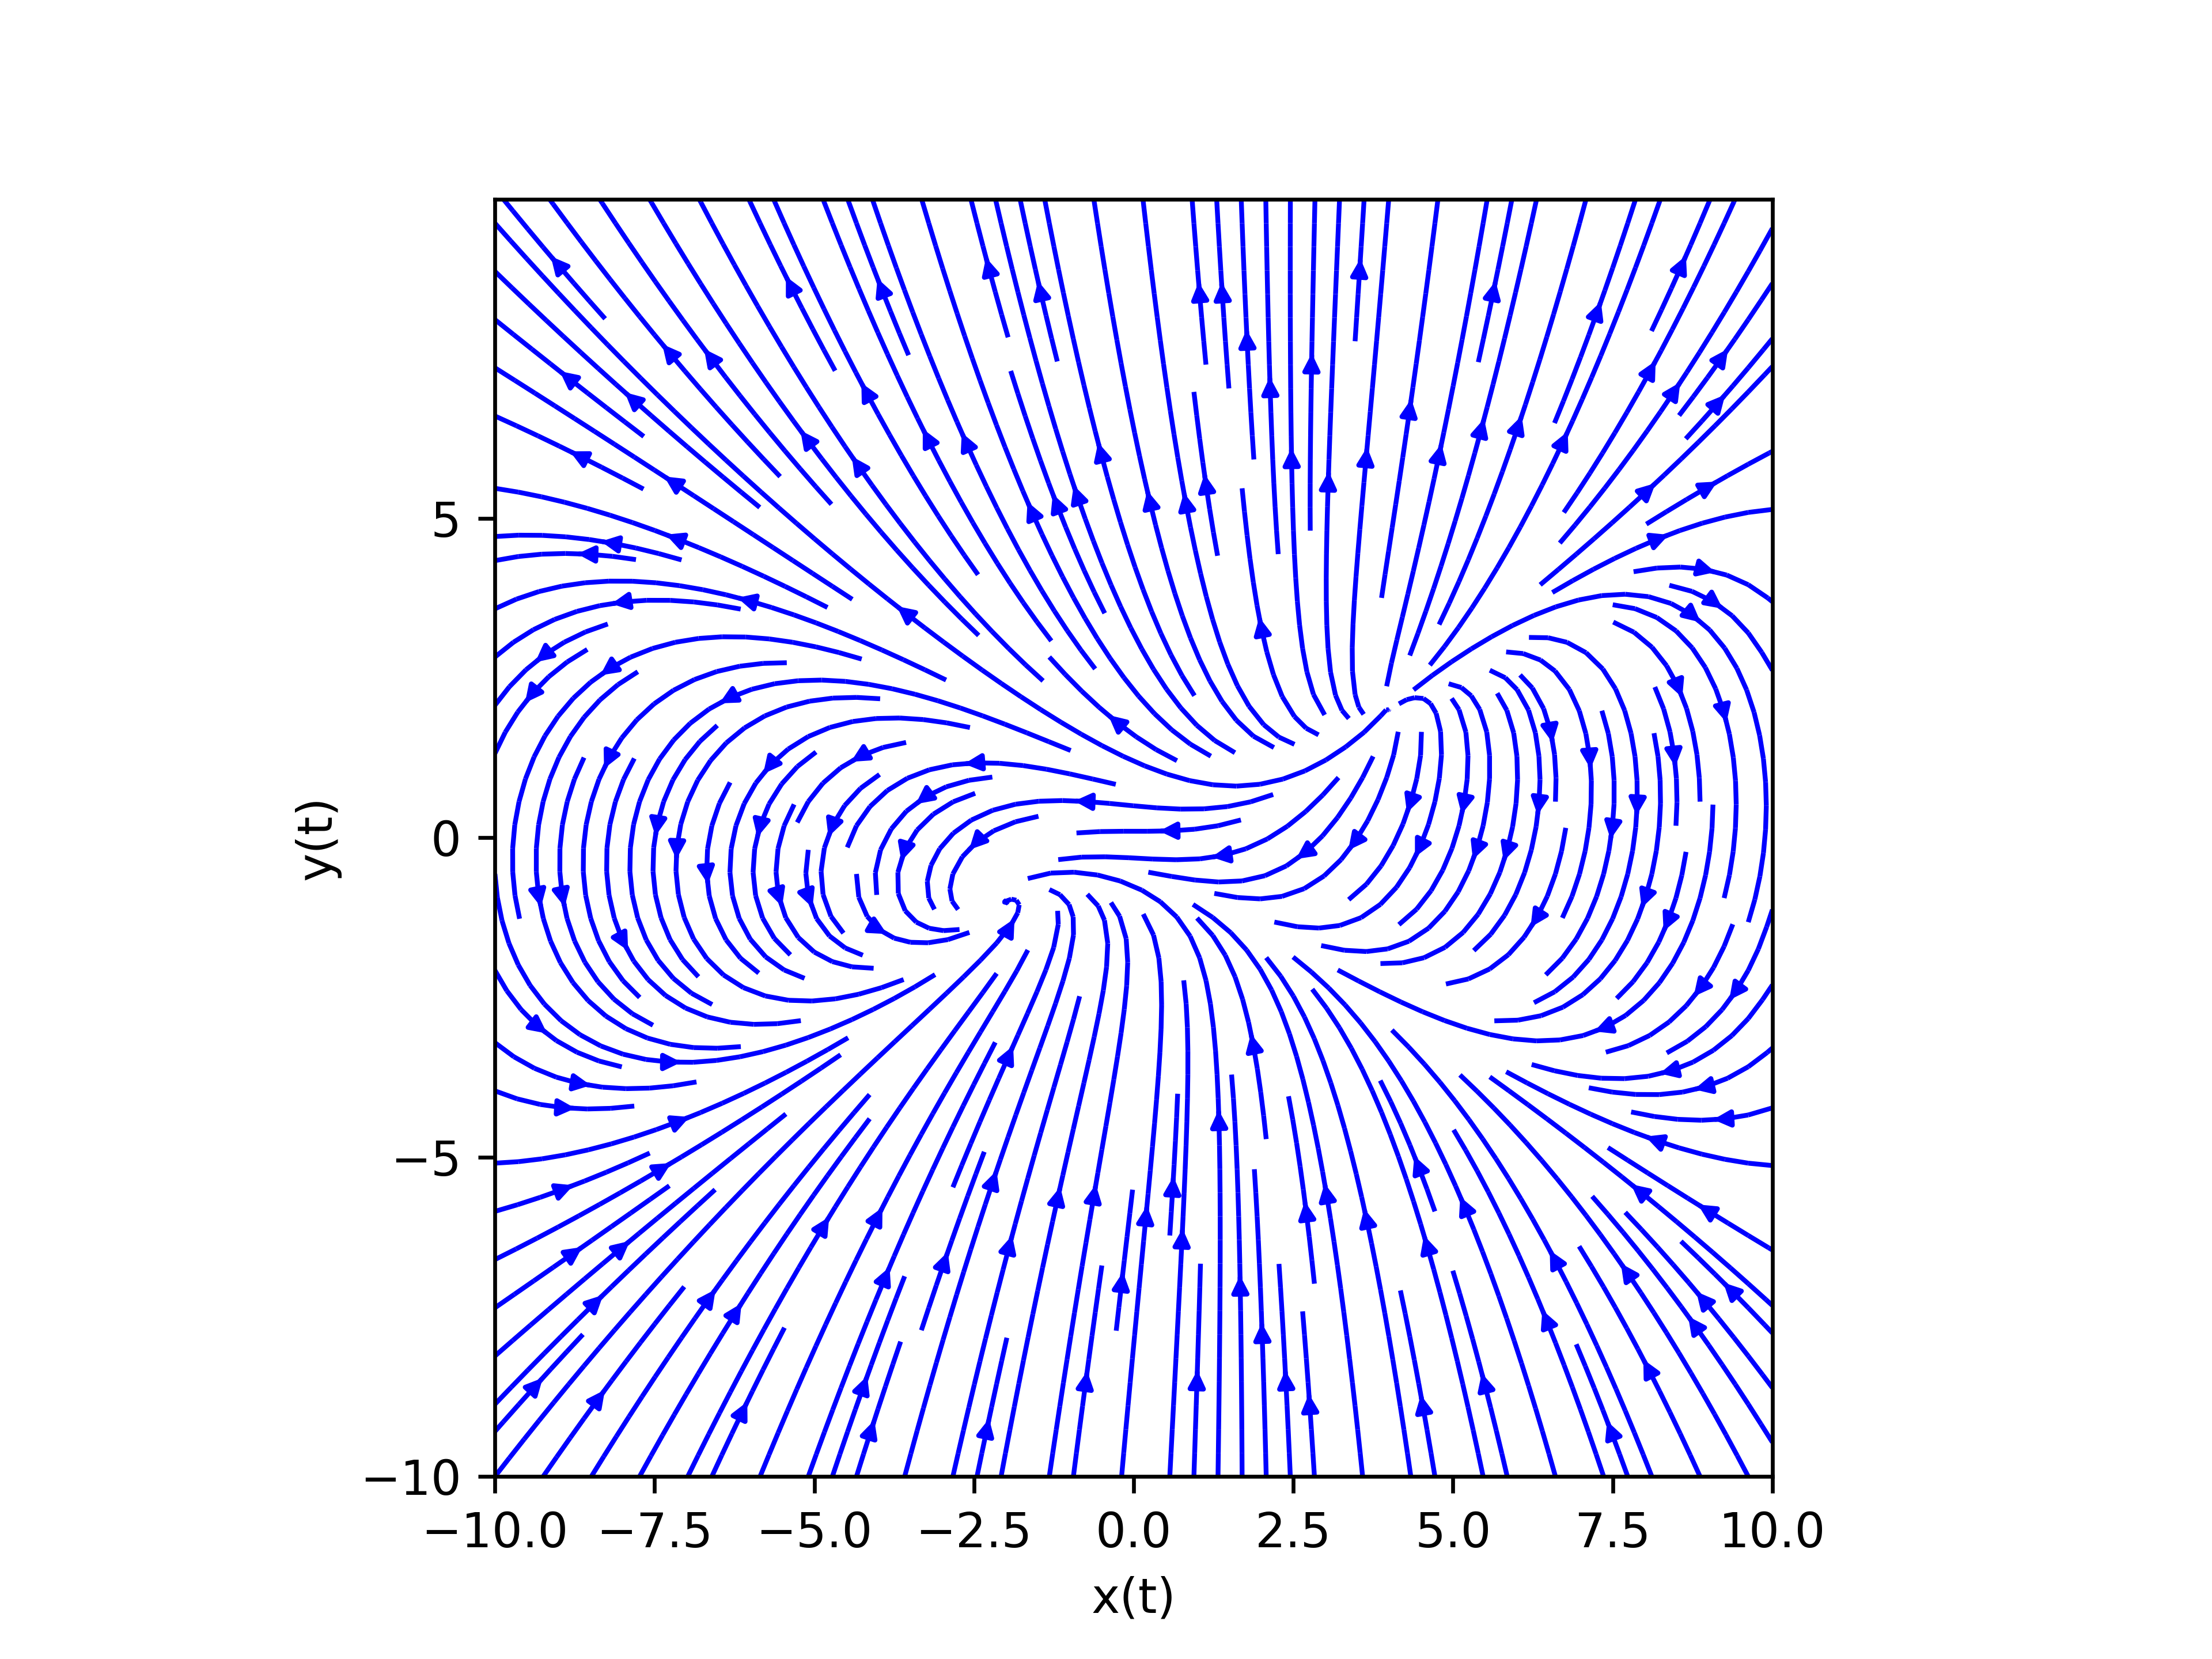
\includegraphics[width=0.78\paperwidth]{graph1_2.png}
    \caption{Фазовый портрет системы \ref{eq:initial2} в виде потоковых линий}
    \label{fig:stream2_1}
\end{figure}
\begin{figure}[h!]
    \centering
    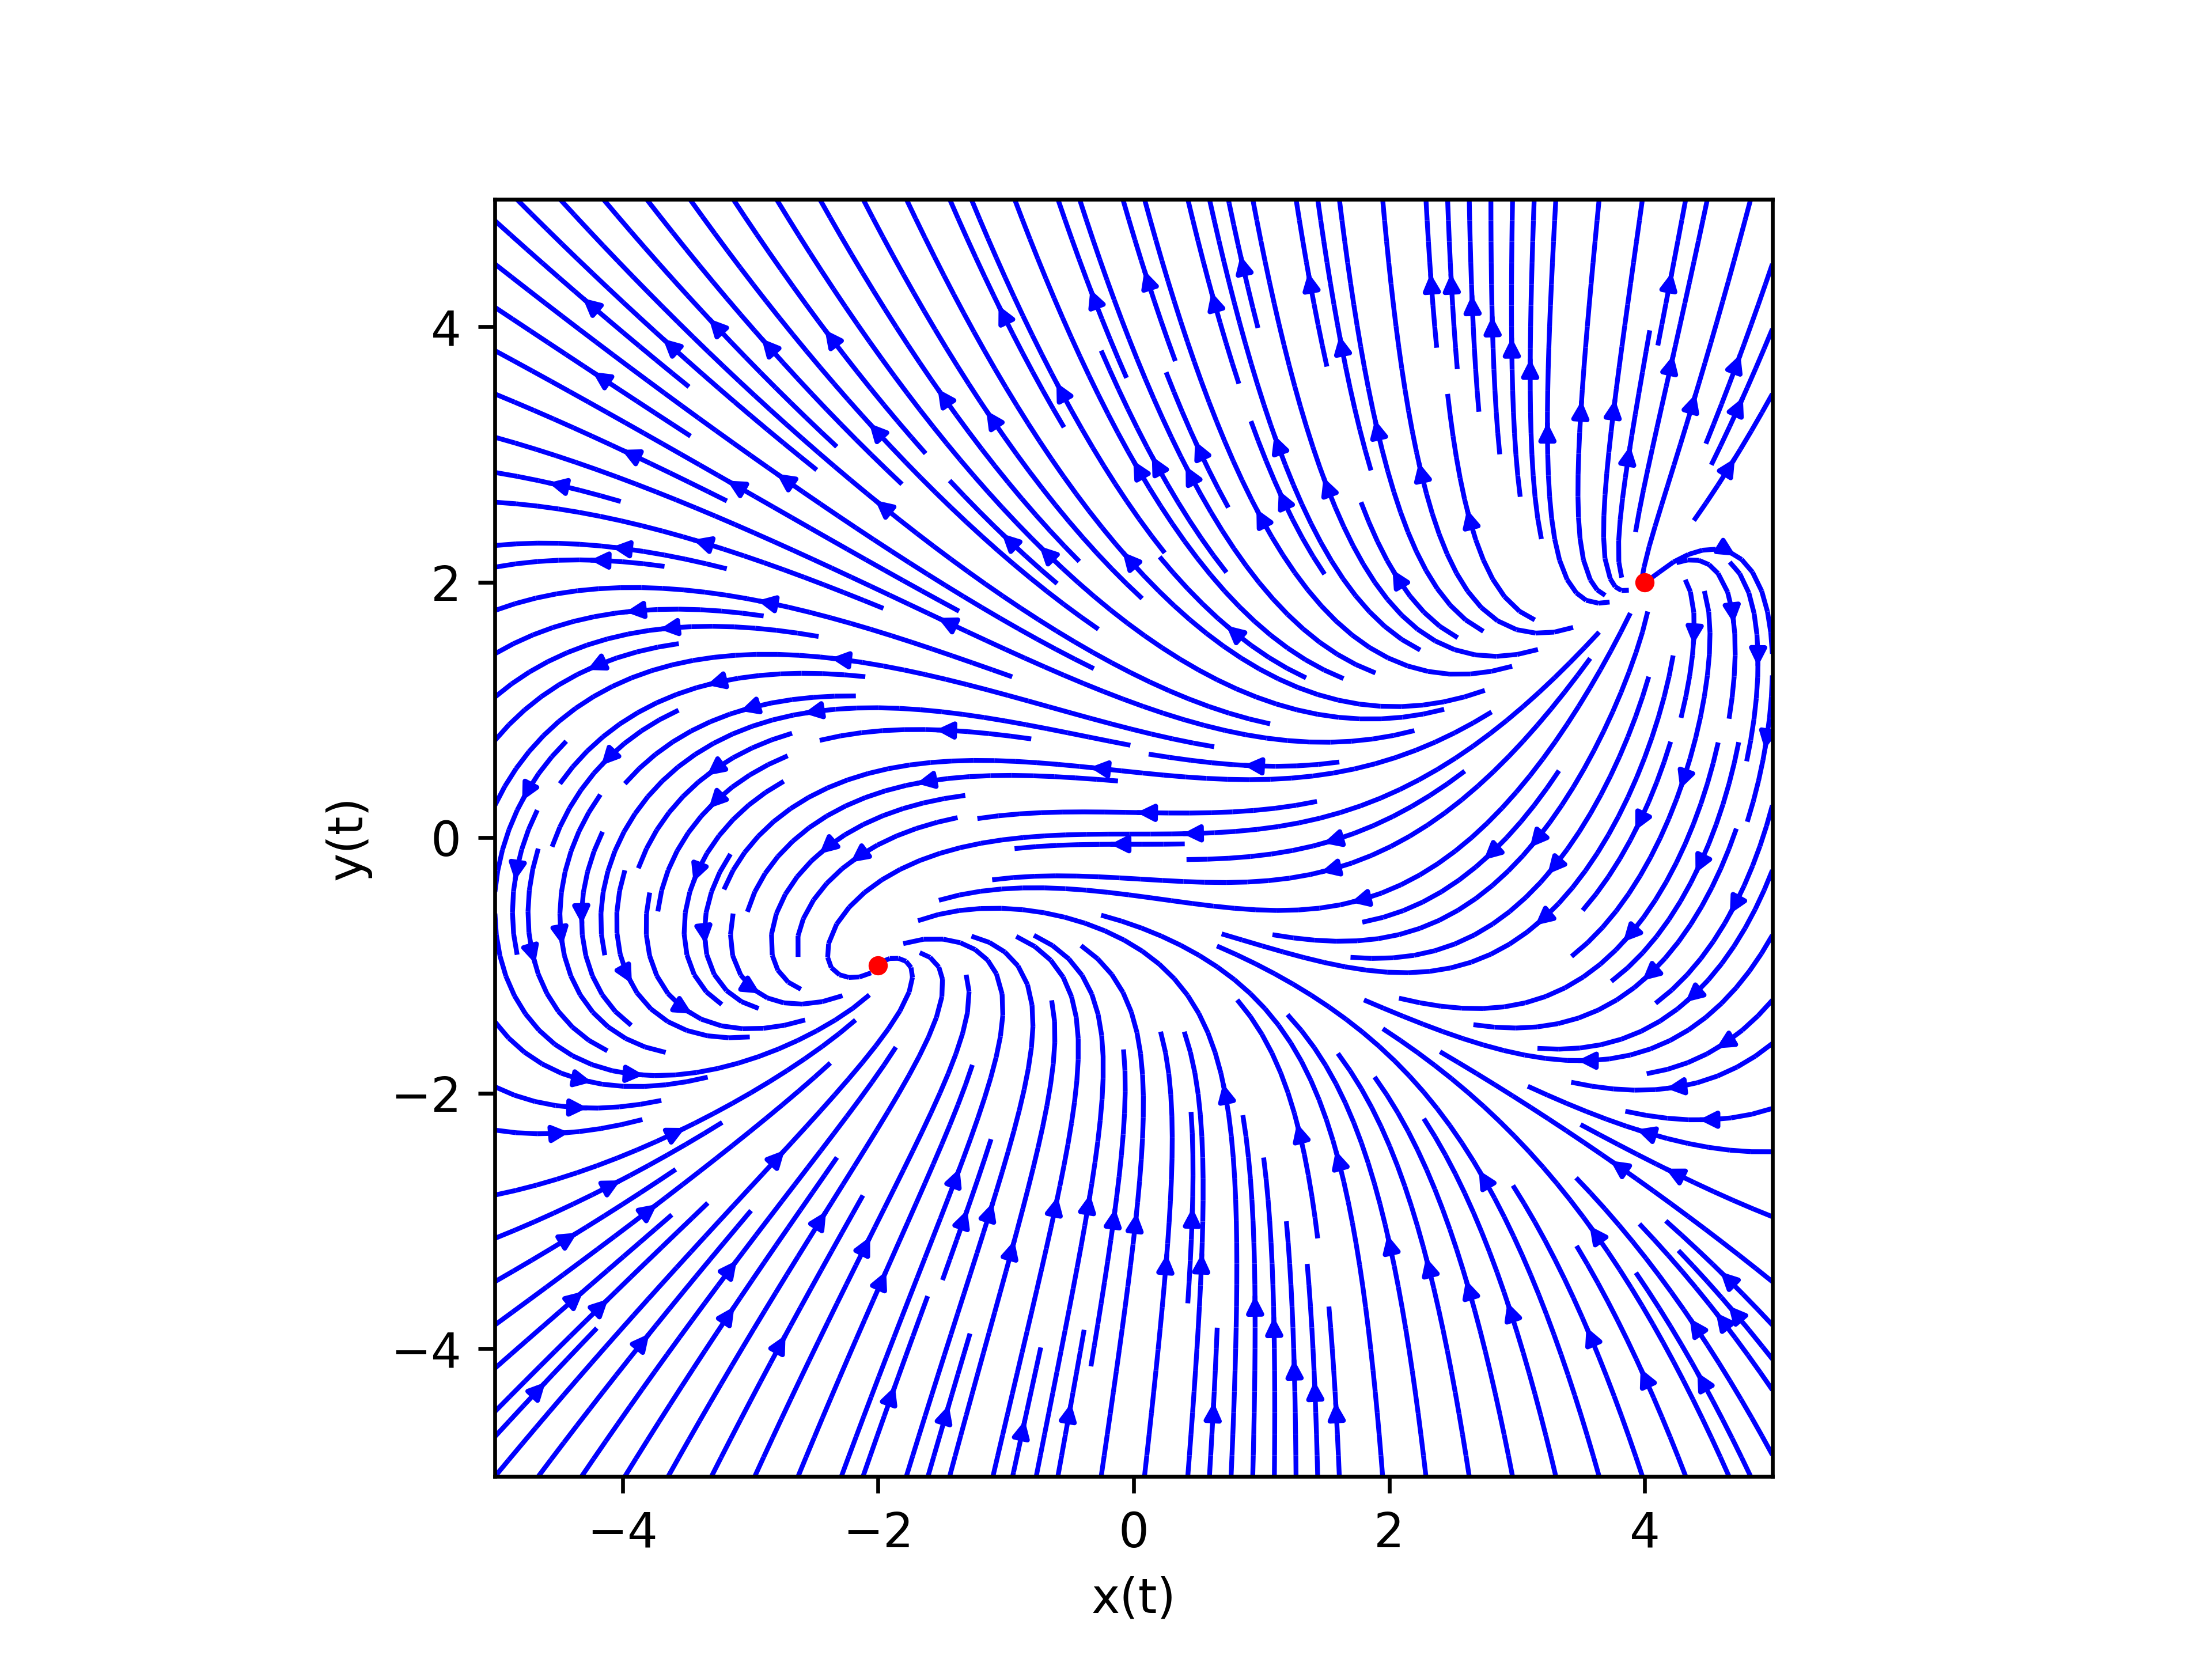
\includegraphics[width=0.78\paperwidth]{graph2_2.png}
    \caption{Фазовый портрет системы \ref{eq:initial2} c отмеченными особыми точками}
    \label{fig:stream2_2}
\end{figure}


\begin{figure}[h!]
    \centering
    \begin{subfigure}{0.4\textwidth}
        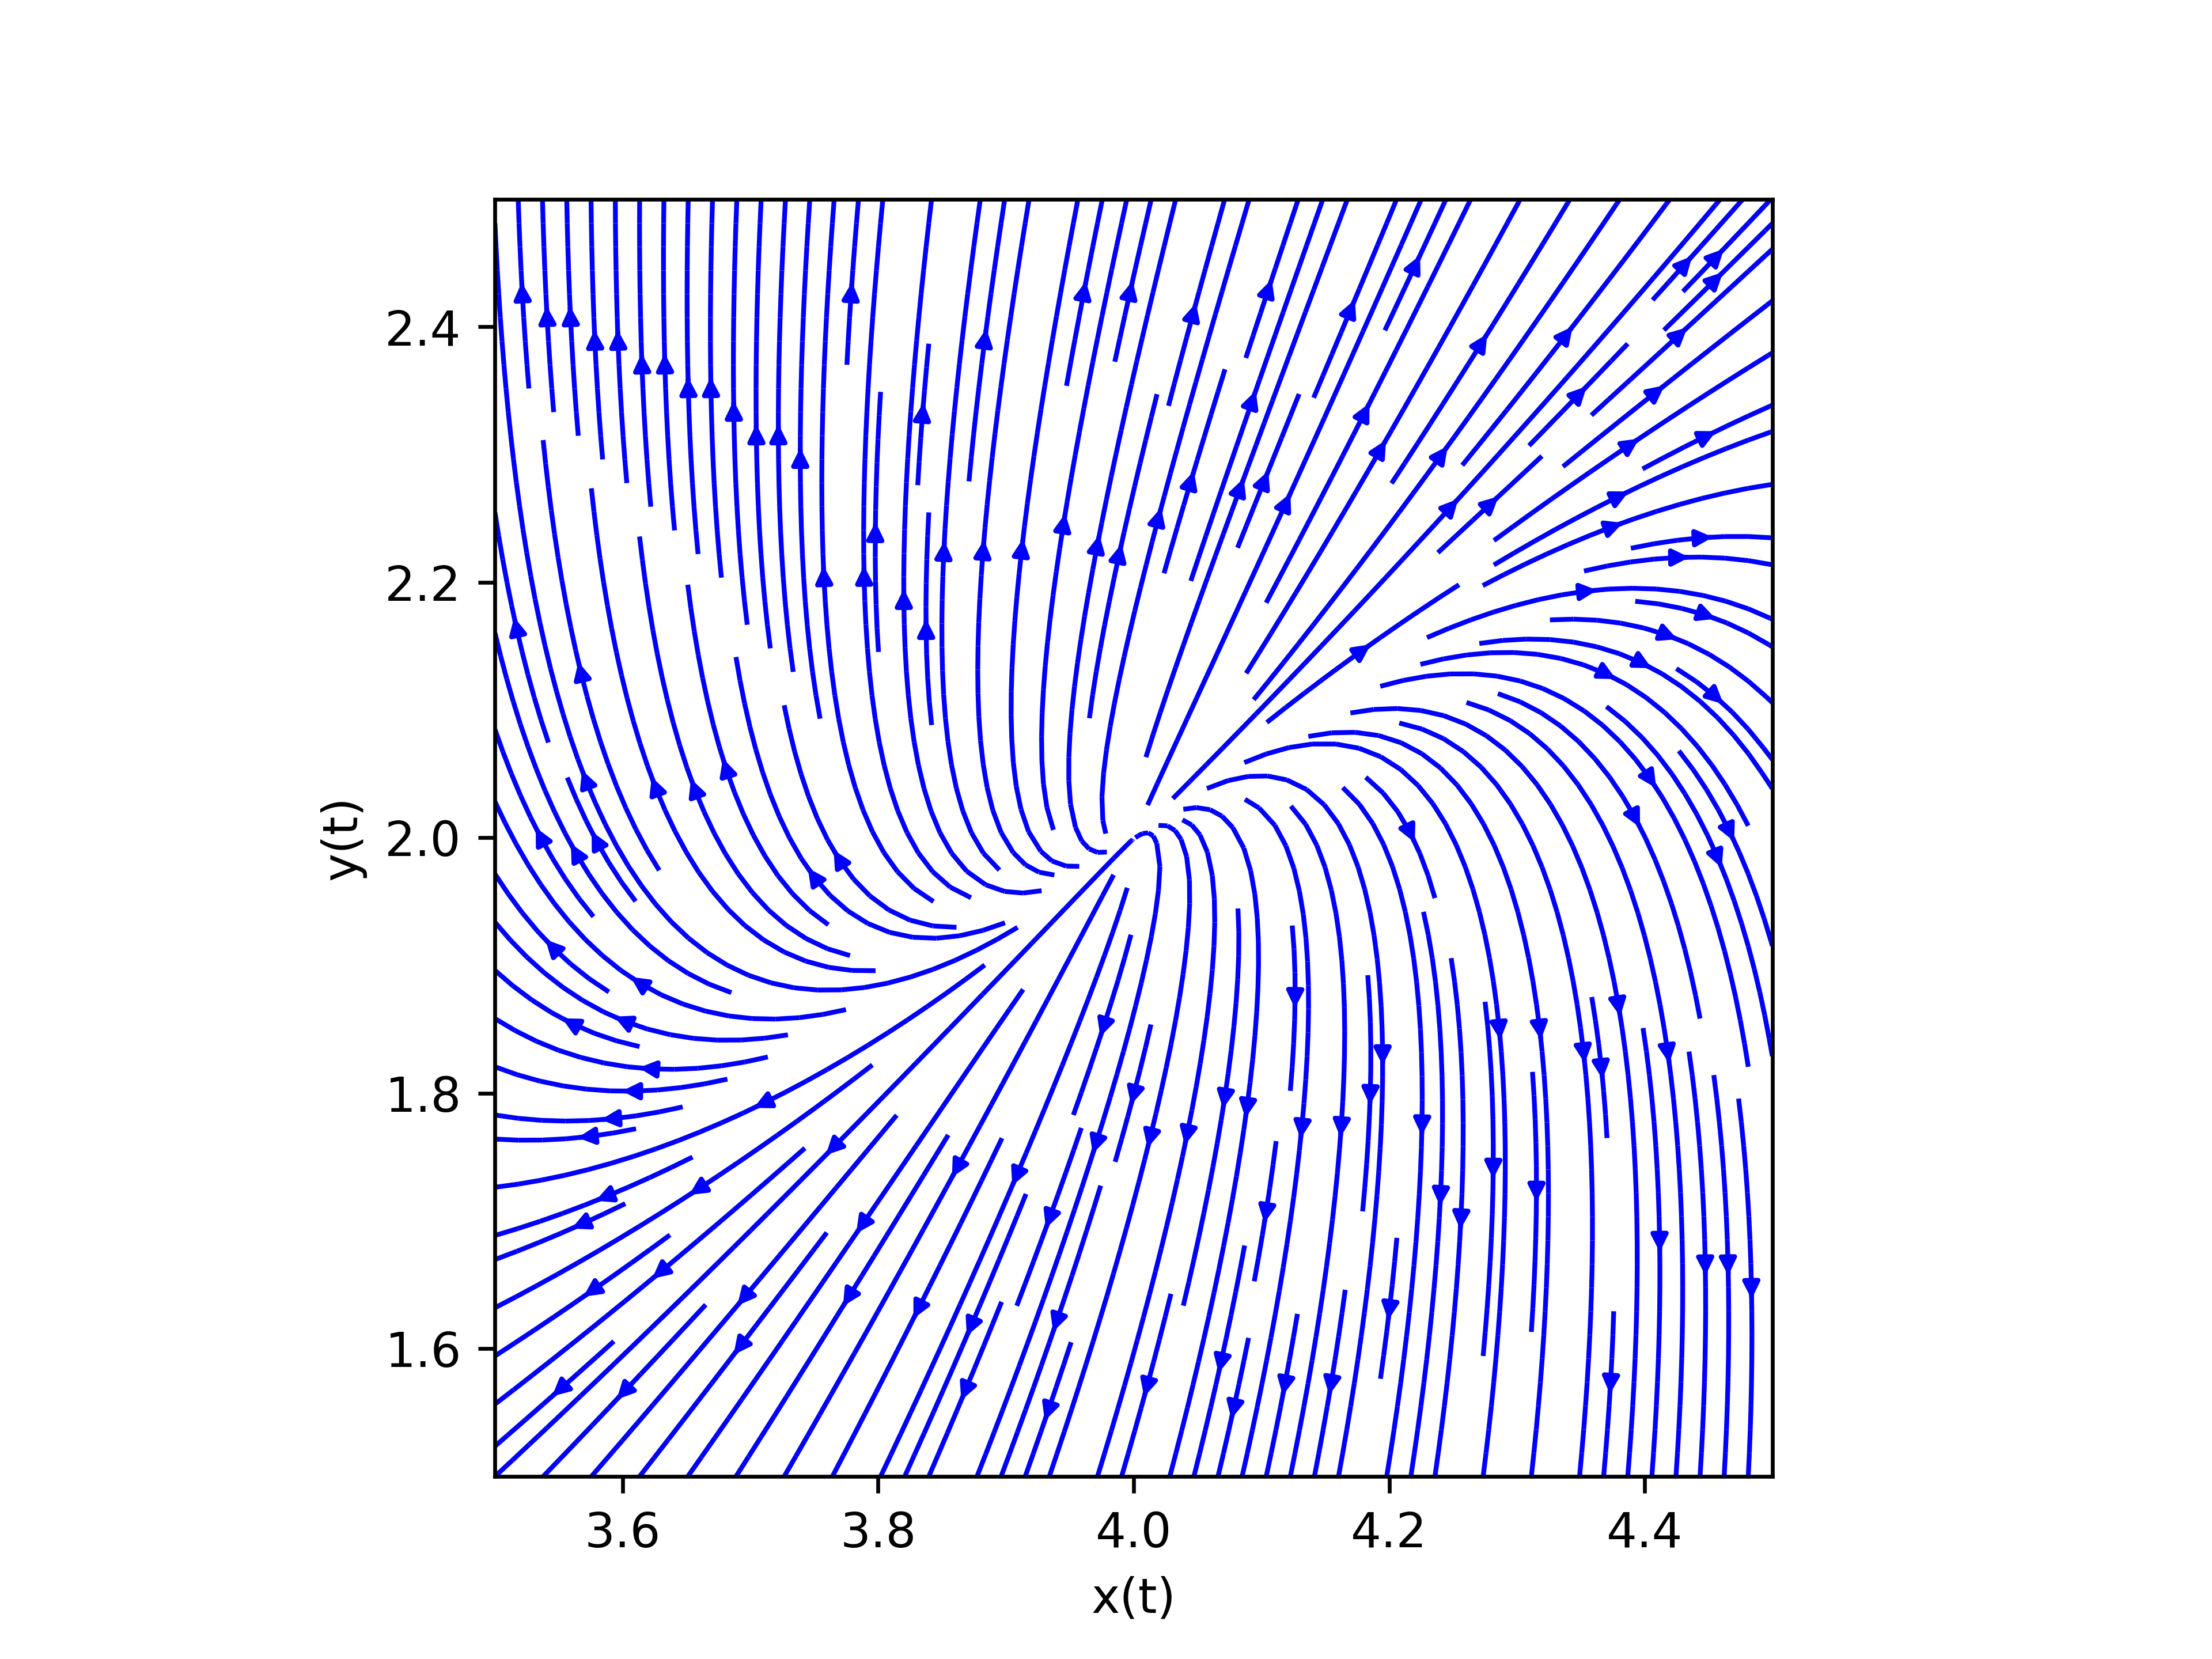
\includegraphics[width=\textwidth]{graph2_A.png}
        \caption{\;Точка $A(4;2)$}
        \label{fig:subfigureA}
    \end{subfigure}
    \begin{subfigure}{0.4\textwidth}
        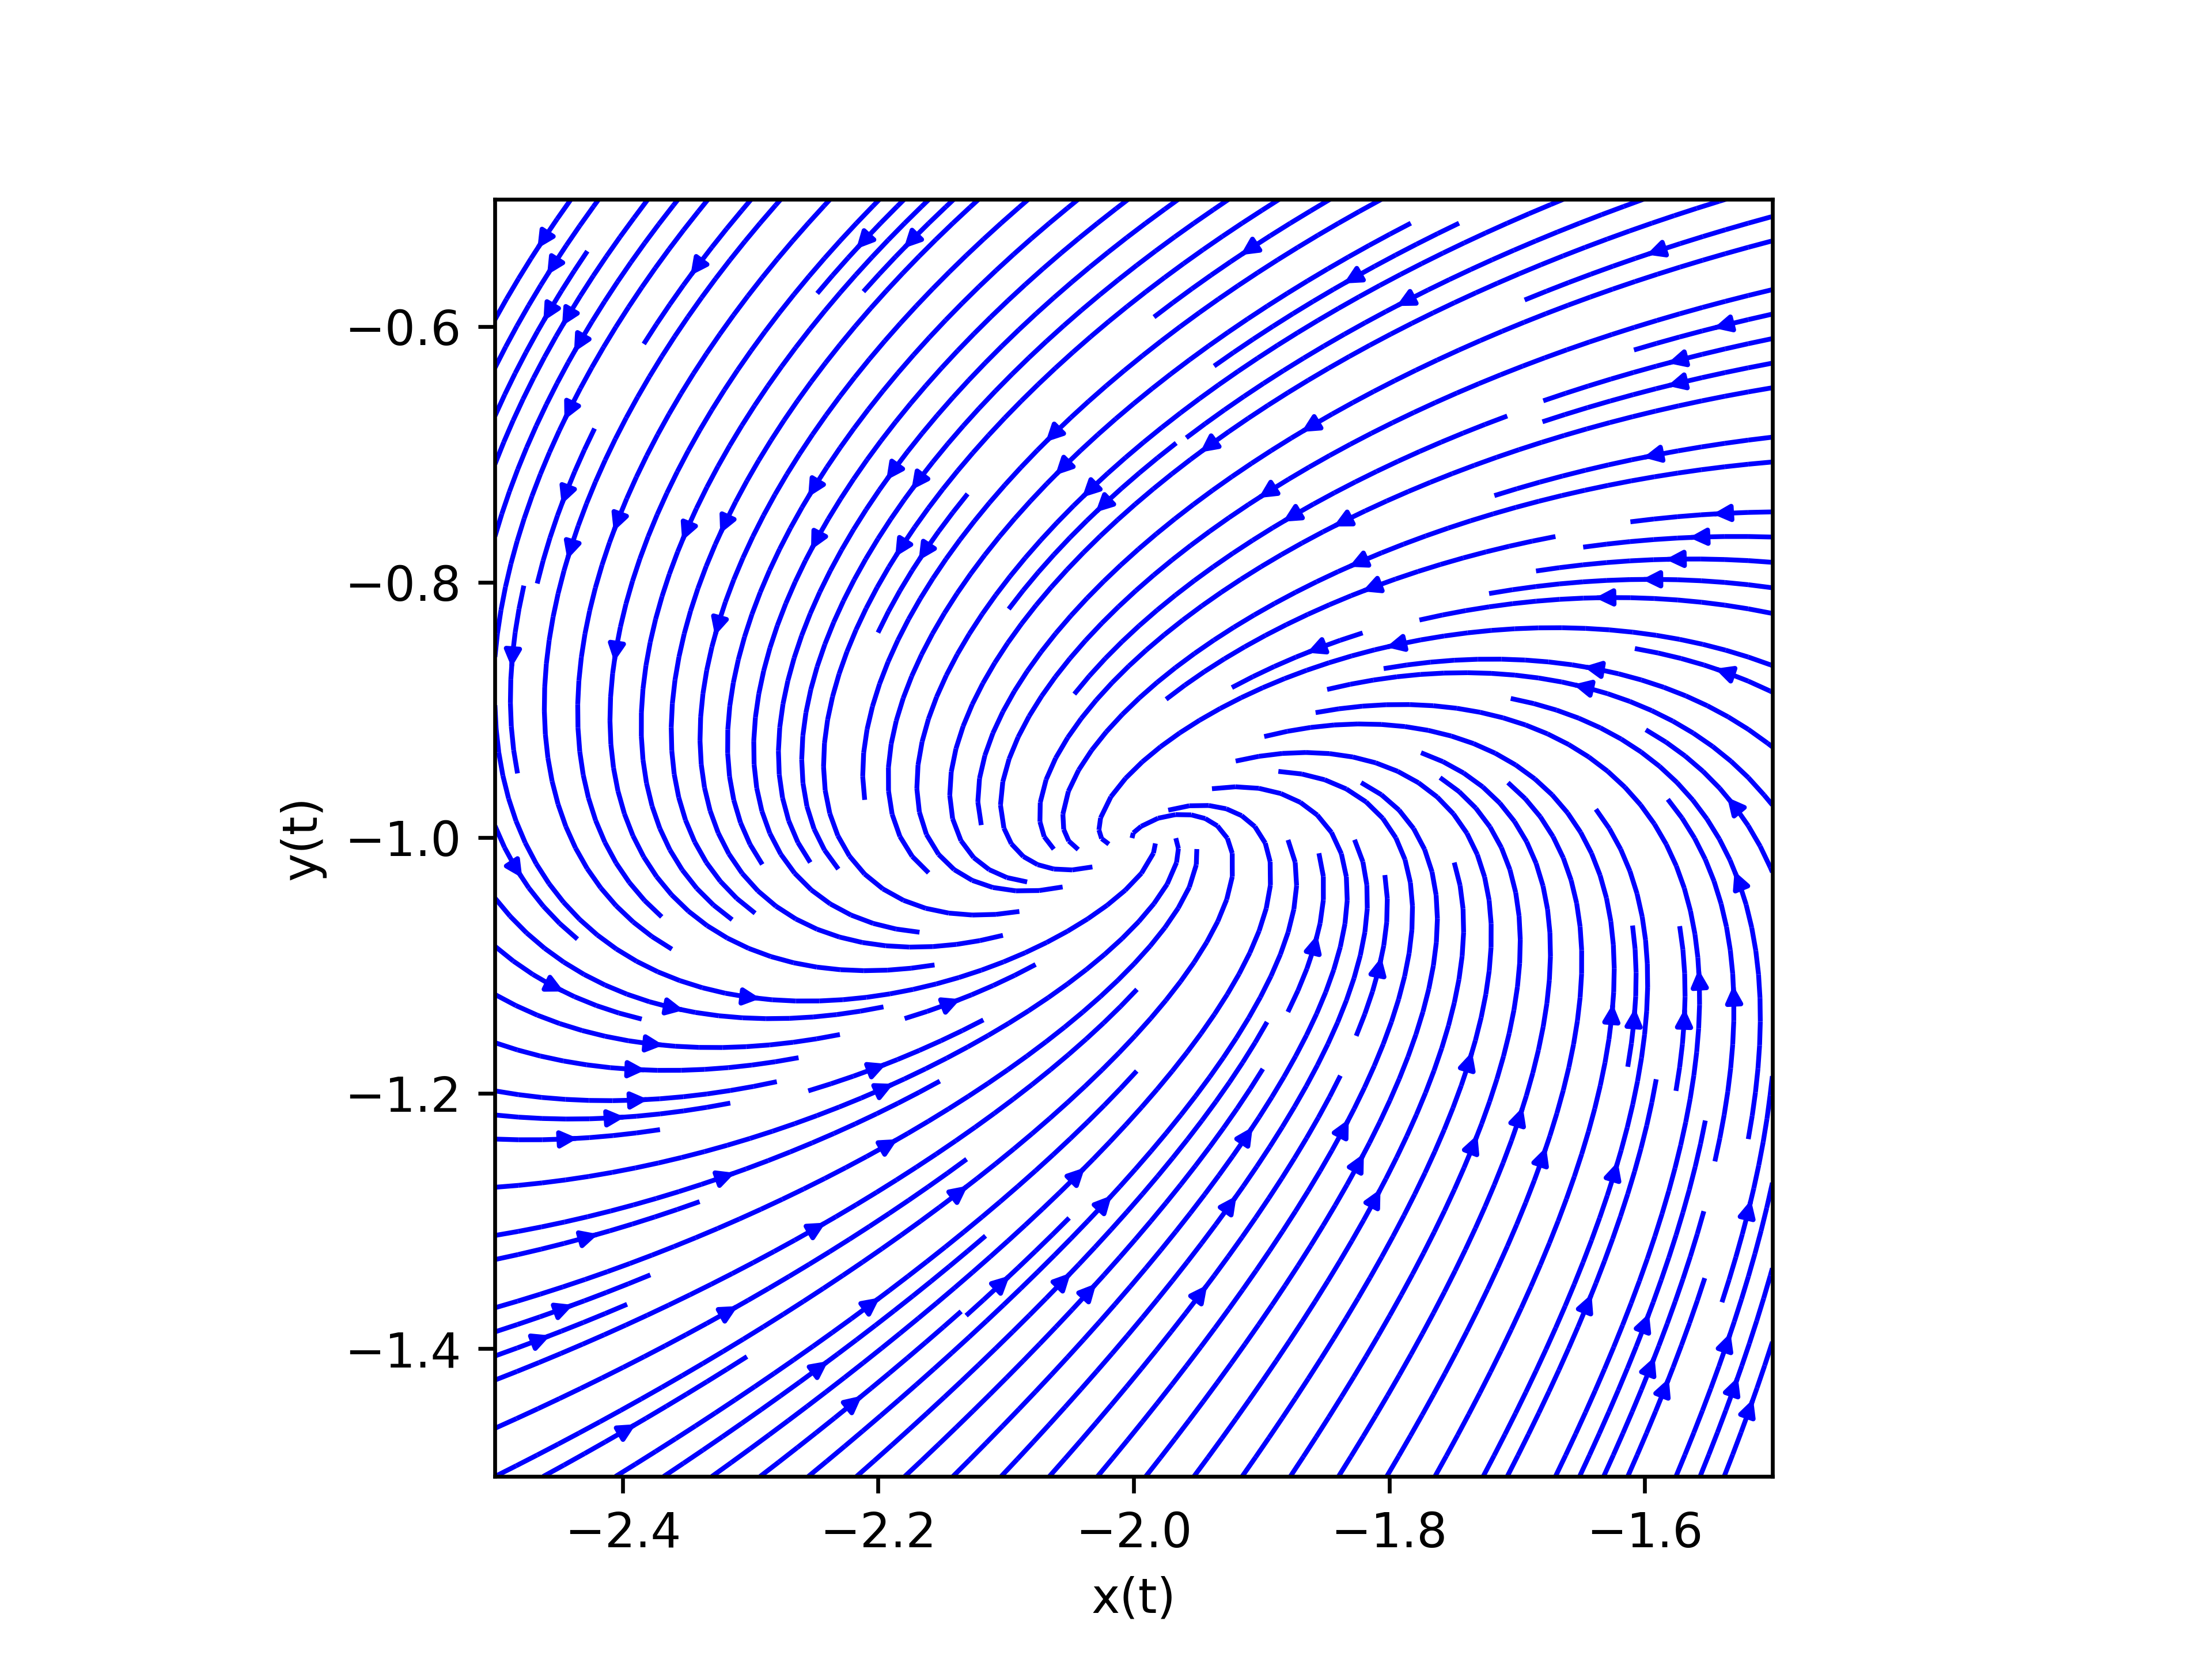
\includegraphics[width=\textwidth]{graph2_B.png}
        \caption{\;Точка $B(-2;-1)$}
        \label{fig:subfigureB}
    \end{subfigure}
    
    \hfill
    \caption{Фазовые портреты системы \ref{eq:initial2} в окрестностях особых точек} 
    \label{fig:combined_graph}
\end{figure}



\newpage

\subsubsection{Представление программного кода}
\vspace{0.3cm}
\begin{lstlisting}[language=Python]
import numpy as np
import matplotlib.pyplot as plt
import math
# Drawing stream type phase portrait of nonlinear ODE system

#Defining the derivatives function
def P_Q(x, y): return [2*x*y-4*y-8, 4*y**2-x**2]

#Calculating the data sets necessary for plotting the first graph
n=1000
X, Y = np.linspace(-10, 10, n), np.linspace(-10, 10, n)
x, y = np.meshgrid(X,Y)
f_x, f_y = np.zeros((n, n)), np.zeros((n,n))
for i in range(n):
    for j in range(n):
        f_x[i, j], f_y[i, j] = P_Q(X[j], Y[i])
        
#Plotting the first graph
plt.streamplot(x, y, f_x, f_y, color='blue', density=1.8, linewidth=1, arrowsize=0.7)
plt.ylabel('y(t)')
plt.yticks(np.arange(-10, 10, step=5))
plt.xlabel('x(t)')
plt.axis('square')
plt.axis([-10, 10, -10, 10])
plt.savefig('graph1_2.png', dpi=600)
plt.show()

#Calculating the data sets necessary for plotting the second graph
X, Y = np.linspace(-5, 5, n), np.linspace(-5, 5, n)
x, y = np.meshgrid(X, Y)
f_x, f_y = np.zeros((n, n)), np.zeros((n, n))
for i in range(n):
    for j in range(n):
        f_x[i, j], f_y[i, j] = P_Q(X[j], Y[i])  
#Plotting the second graph
plt.streamplot(x, y, f_x, f_y, color='blue', density=2.0, linewidth=1, arrowsize=0.7)
plt.plot(4,2,'r.')
plt.plot(-2,-1,'r.')
plt.ylabel('y(t)')
plt.xlabel('x(t)')
plt.axis('square')
plt.axis([-5, 5, -5, 5])
plt.savefig('graph2_2.png', dpi=600)
plt.show()


#Plotting the A subraph
X, Y = np.linspace(3.5, 4.5, n), np.linspace(1.5, 2.5, n)
x,y = np.meshgrid(X, Y)
f_x, f_y = np.zeros((n,n)), np.zeros((n,n))
for i in range(n):
    for j in range(n):
        f_x[i, j], f_y[i, j] = P_Q(X[j], Y[i])
plt.streamplot(x, y, f_x, f_y, color='blue', density=1.8, linewidth=1, arrowsize=0.7)
plt.ylabel('y(t)'); plt.xlabel('x(t)')
plt.axis('square')
plt.axis([3.5, 4.5, 1.5, 2.5])
plt.savefig('graph2_A.png', dpi=600)
plt.show()

#Plotting the B subraph
X, Y = np.linspace(-2.5, -1.5, n), np.linspace(-1.5, -0.5, n)
x, y = np.meshgrid(X,Y)
f_x, f_y = np.zeros((n, n)), np.zeros((n, n))
for i in range(n):
    for j in range(n):
        f_x[i, j], f_y[i, j] = P_Q(X[j], Y[i])
plt.streamplot(x, y, f_x, f_y, color='blue', density=1.8, linewidth=1, arrowsize=0.7)
plt.ylabel('y(t)'); plt.xlabel('x(t)')
plt.axis('square')
plt.axis([-2.5, -1.5, -1.5, -0.5])
plt.savefig('graph2_B.png', dpi=600)
plt.show()


\end{lstlisting}

\newpage


\section{Замечания к построению фазовых портретов}
Для линейной системы ДУ: так как единственная особая точка системы — \textbf{седло} в начале координат, представленный на Рис. \ref{fig:stream1_1}, то невозможно задать произвольную область построения и выбрать на её границе случайное множество точек, из которых будут проведены к положению равновесия фазовые траектории. \par
Для нелинейной системы ДУ: в случае точки $A$ система будет неустойчива и  направление касательных векторов в её окрестности будет соответствовать движению от положения равновесия. Точка $B$ — асимптотически устойчива, а значит направление любого касательного вектора, находящегося в окрестности точки $D$, будет соответствовать движению к положению равновесия. Таким образом, для построения фазового портрета достаточно рассмотреть некоторое множество начальных точек, находящихся на границе рассматриваемой области.
\vspace{1.5cm}

\section{Заключение}
Найдя особые точки линейной \ref{eq:initial1} и нелинейной \ref{eq:initial2} систем дифференциальных уравнений и построив их фазовые портреты в области, содержащей эти точки, мы получили детальное представление о поведении решений этих систем вблизи положений равновесия и узнали какую форму  приобретают при тех или иных начальных условиях и при малых отклонениях от точки равновесия траектории материальных точек, движение которых на практике могут описывать данные уравнения.\par
Кроме того, данная работа позволила нам лучше осознать теорию устойчивости по Ляпунову. Так, работа над построением фазовых портретов дала более фундаментальное понимание концепции устойчивости и дала возможность самостоятельно построить и осознать визуальные примеры поведения решений в окрестностях особых точек разного характера.\par
Наконец, эта работа предоставила возможность попрактиковаться в решении систем дифференциальных уравнений, а также дала нам чёткое представление о графическом представлении решений систем дифференциальных уравнений при помощи графических библиотек, представленных в Python.
\newpage

\begin{thebibliography}{9} \large
\bibitem{book01} Асташова И. В., Никишкин В. А., \textit{Практикум по курсу «Дифференциальные уравнения». Учебное пособие}, Изд. 3–е, исправленное.—М.: Изд. центр ЕАОИ, 2010.
\bibitem{book02} Филиппов А. Ф., \textit{Введение в теорию дифференциальных уравнений: Учебник}, -М.: Изд. Едиториал УРСС, 2004. - 240 с.
\bibitem{book03} NumPy, URL: \verb!https://numpy.org/!. (Дата обращения: 15.05.2024)
\bibitem{book04} Matplotlib: Visualization with Python, URL: \verb!https://matplotlib.org/!. (Дата обращения: 14.05.2024)
\bibitem{book05} Carlisle D., \textit{The longtable package.}, Version number v4.17, 2021-09-01, URL: \verb!http://mirrors.ibiblio.org/CTAN/macros/latex/required/tools/longtable.pdf!. (Дата обращения: 14.05.2024)
\end{thebibliography}
\begin{center}
\LaTeX
\end{center}

\end{document}